\documentclass[a4paper]{report}

\usepackage[english]{babel}
\usepackage{amsmath}
\usepackage{graphicx}
\usepackage{subcaption}

\author{Maarten de Jonge \\
        Inge Becht}
\date{\today}
\title{Various Models and Simulations}

\begin{document}
\maketitle

\chapter{Simulating a forest fire with a cellular automaton}
\label{cha:ff}

\section{Implementation} 
\label{sec:ff_impl}

The simulation is implemented as a cellular automaton using the following simple
rules:
\begin{enumerate}
    \item A cell can be empty, vegetated, burning, or burnt.
    \item A vegetated cell will become burning if one of its neighbours is
          burning.
    \item A burning cell will become burnt.
\end{enumerate}
where ``neighbour'' is defined as being in the 8-cell Moore-neighbourhood of a
cell and rules 2 and 3 govern the transition from one moment in time to the
next.

The playing field gets initialised with a certain vegetation density, which
gives the probability of each individual cell starting out in the vegetated
state (a cell starts out vegetated if $Q <= D$ where $D$ is the vegetation
density and $Q$ is a random float between 0 and 1). The entire bottom row will
be set on fire initially (regardless of the content of the cells). The
simulation runs until there are no more burning cells.

% section ff_impl (end)

\section{Experimentation} 
\label{sec:ff_exp}

After each run of the simulation, the following data was collected:
\begin{itemize}
    \item Whether the other side of the field (the top-side, since the fire
        starts at the bottom) had been reached.
    \item How many steps it took to the other side (0 if it wasn't reached).
    \item The percentage of vegetation that was burnt.
\end{itemize}

The simulation has been run 250 times with the parameter tuples $(FieldSize,
Density)$, where $FieldSize \in \{10, 15, 20, 25, 30, 35\}$ and \\
$Density \in \{0.05, 0.1, 0.2, 0.3, 0.4, 0.5, 0.6, 0.7, 0.8, 0.9\}$, leading to
$6 \times 10$ trials being run 250 times each. The field
was chosen to be square, leading to a $FieldSize \times FieldSize$ sized field.

The results were plotted as heatmaps because of the large amount of overlapping
points, and are shown in figures \ref{fig:reached}, \ref{fig:steps} and
\ref{fig:burnt}.

\begin{figure}[htbp]
    \centering
    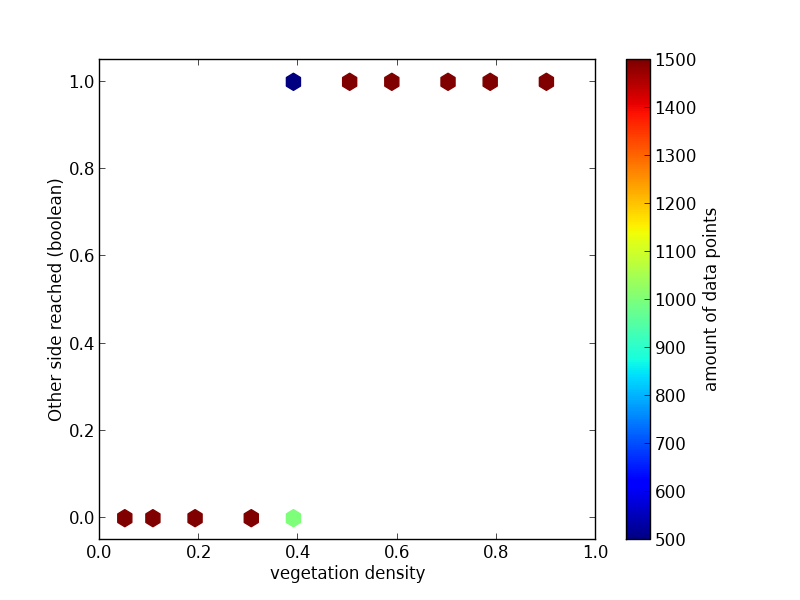
\includegraphics[width=0.7\textwidth]{./density_vs_reached.png}
    \caption{A boolean plot showing whether the other side was reached (1 =
             reached, 0 = not reached)}
    \label{fig:reached}
\end{figure}

\begin{figure}[htbp]
    \centering
    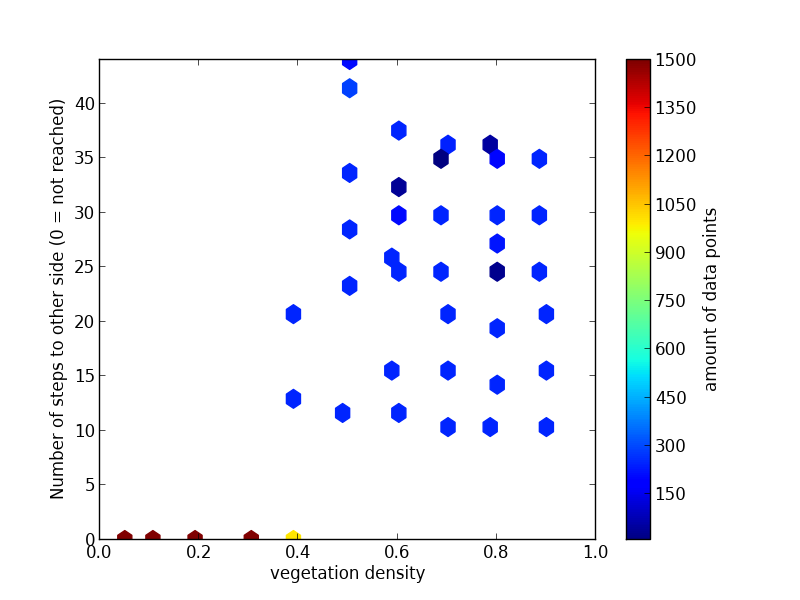
\includegraphics[width=0.7\textwidth]{./density_vs_steps.png}
    \caption{Number of steps to reach the other side as function of the density.
             A value of 0 means the other side wasn't reached.}
    \label{fig:steps}
\end{figure}

\begin{figure}[htbp]
    \centering
    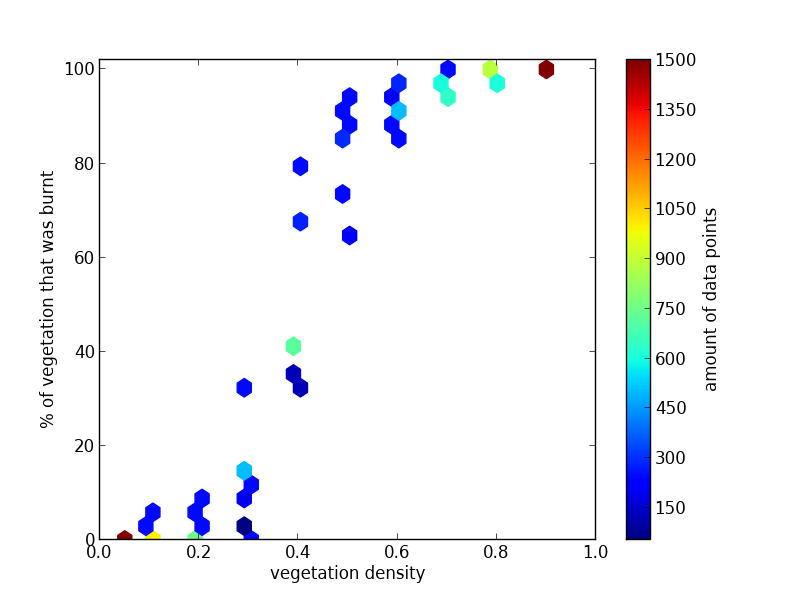
\includegraphics[width=0.7\textwidth]{./density_vs_burnt.png}
    \caption{Percentage of burnt trees as function of the density.}
    \label{fig:burnt}
\end{figure}

\begin{figure}[htbp]
    \centering
    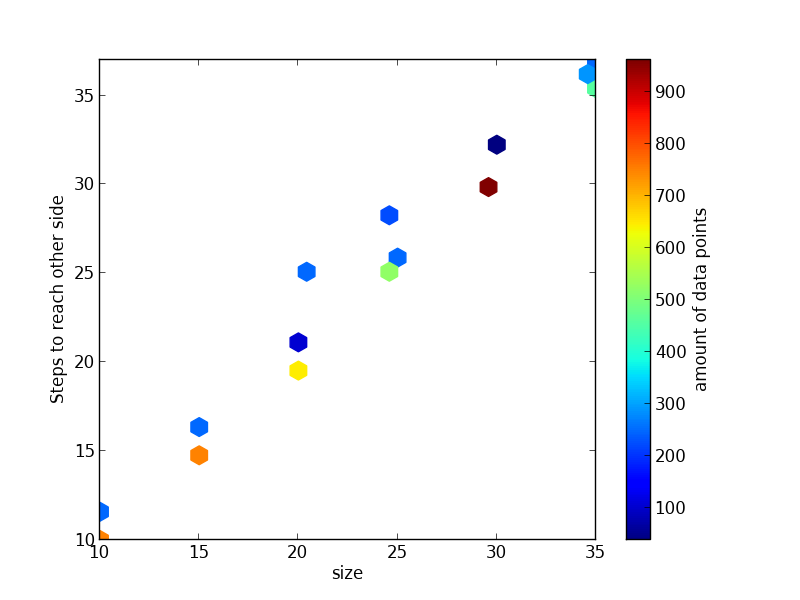
\includegraphics[width=0.7\textwidth]{./size_vs_steps.png}
    \caption{Field size vs steps to other side, restricted to densities of [0.6,
    \label{fig:size}
0.9]}
\end{figure}


% section ff_exp (end)

\section{Results} 
\label{sec:ff_results}

Looking at the reaching of the other side, there's clearly a hard threshold
around a density of $0.4$. Below $0.4$ none of trials reach the other side, while
above it 100\% of the trials reach it. At $0.4$ it varies, with a majority of
trials not reaching the other side.

The steps required to reach the other side looks to be roughly evenly divided
between 10 and 40 steps at densities of $0.6$ and up, with a slightly higher
boundary (45) at a density of $0.5$. Keeping in mind that the simulation was run
at various different sizes for the field, it is reasonable to suspect that this
has an influence on the required steps to reach the other side. To be sure of
this, the fieldsize has been plotted against the required steps, filtered for
densities from 0.6 to 0.9 (figure \ref{fig:size}). This shows that in general,
it takes about $n$ steps for the fire to get to the other side of an $n \times
n$ field, sometimes slightly more.

The percentage of burnt trees increases with a roughly S-shaped curve, with the
percentage quickly increasing with the middle densities, and more slowly at the
extremes, culminating at a (practically) 100\% burn rate at a density of $0.9$.

% section ff_results (end)

\section{Conclusion} 
\label{sec:ff_conc}

The act of fire reaching the other side displays a threshold effect around a
density of $0.4$ - $0.5$. A density of $0.5$ is enough for the fire to reach the
other side in every trial, and from $0.6$ on it is generally reached in the
minimum possible amount of steps.

The percentage of burnt trees acts a bit more sigmoid-like, displaying an
S-shaped curve from 0\% to 100\%.

Thus, if you want to burn down a forest and get the fire to the other side, the
density of the forest doesn't matter as long it's over $0.5$. However if you
hate nature and want to burn down as much forest as possible, pick the forest
with the highest density.

% section ff_conc (end)

% chapter ff (end)

\chapter{A grid-simulation of the spread of malaria}
\label{cha:malaria}

In this grid-simulation a representation is made of how malaria can spread
throughout a small population of humans and how well it can flourish
depending on human and mosquito density. 

The spread of malaria is quite complex and is simplified for this
grid-simulation. The following assumptions are made for this simulation:

\begin{itemize}
    \item A human can be susceptible, infected, immune or dead. None of the states are
        permanent except for death.
    \item A mosquito can be susceptible, infected or dead. 
    \item Mosquitoes can move to neighbouring cells. All mosquitoes make a
        random move if possible, and else stay where they are.
    \item Humans are stoic.
    \item Only one mosquito can occupy a cell at a time iteration, but both a
        human and a mosquito can be in the same cell.
    \item Both humans and mosquitoes can die and for every died person or
        mosquito a new uninfected one is born.
    \item Humans will spawn next to an already existing human, and the same for
        mosquitoes (creating clusters).
    \item If a susceptible mosquito bites an infected human it changes to the
        infected state. If a infected mosquito bites an uninfected human it
        changes the human to the infected state. All other cases won't change
        the states.
    \item In the first state all cells contain exactly one or none elements. So
    if a simulation has dimension $n \times m$, than the amount of elments can
    at max be $n \times m$
    \item Each time iretation the mosquitoes move one space, people change state
        (new ones spawn)
        and people can get bitten.
    \item The grid is not a torus but a bounded rectangle. This because of
        implementation simplicitity, but seems more like real life as well.
\end{itemize}

\begin{figure}[htbp]
    \centering
    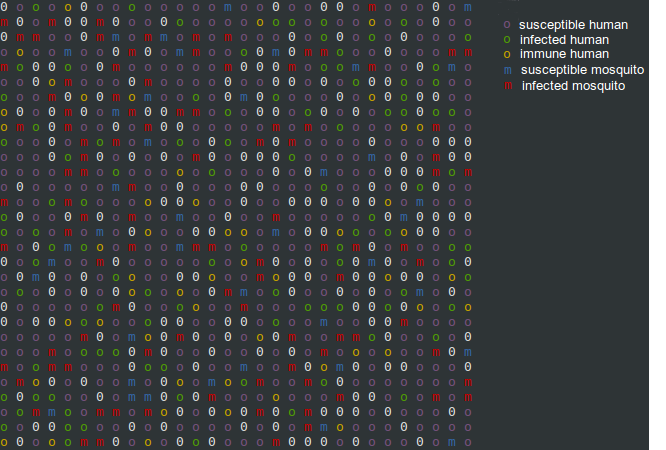
\includegraphics[width=1\textwidth]{malaria_ascii.png}
    \caption{A visualtion of the initial state of the grid simulation. }
    \label{fig:ascii}
\end{figure}

Every iteration all mosquitoes make a random move towards a neighbouring cell,
the state of humans is updated to

The grid is not implemented as a thorus due to ease of implementation and not
making things easier to simulate

Table \ref{tab:rates} shows the rates used while the experimentations were made
with the malaria grid. Some experimentations were made to come to these values,
but is not the subject of the experimentation


\begin{table}
\centering
\begin{tabular}{|l|l|r|}
        \hline
        variable&for&rate\\
        \hline
        deathrate&susceptible humans &0.003\\
        deathrate&infected humans&0.03\\
        deathrate&immune humans&0.003\\
        deathrate&susceptible mosquitoes&0.045\\
        deathrate&infected mosquitoes&0.045\\
        turning susceptible&immune humans& 0.06\\
        hungry&infected mosquito  & 0.3\\
        hungry&uninfected mosquito& 0.3\\
        infectionrate&infected mosquito& 1\\
        \hline
\end{tabular}
\caption{Rates used for experimentations }
\label{tab:rates}
\end{table}





For the following experiments a 30 X 30 grid was used in which experimentations
were made with the human density and mosquito density and the amount of
susceptible and unsusceptible humans that were started with


% chapter malaria (end)

\end{document}
